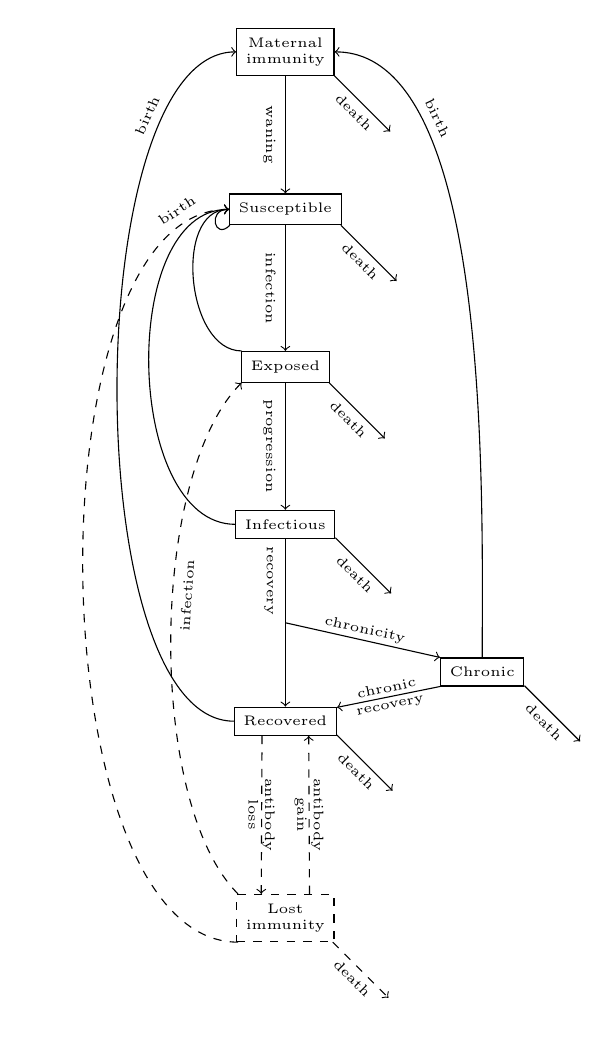
\begin{tikzpicture}[compartment/.style = {rectangle, draw}, font=\fontsize{5pt}{6}\selectfont]
  % Compartments.
  \node at (0, 11) [compartment, align=center, name=MaternalImmunity] {Maternal\\immunity};
  \node at (0, 9) [compartment, name=Susceptible] {Susceptible};
  \node at (0, 7) [compartment, name=Exposed] {Exposed};
  \node at (0, 5) [compartment, name=Infectious] {Infectious};
  \node at (2.5, 3.125) [compartment, name=Chronic] {Chronic};
  \node at (0, 2.5) [compartment, name=Recovered] {Recovered};
  \node at (0, 0) [compartment, align=center, dashed, name=Partial] {Lost\\immunity};

  % Location for branch from Infectious to Chronic and Recovered.
  \coordinate (recovery) at (0, 3.75);

  % Infection-related processes.
  \draw [->] (MaternalImmunity)
             to node [rotate=-90, below] {waning}
             (Susceptible);
  \draw [->] (Susceptible)
             to node [rotate=-90, below] {infection}
             (Exposed);
  \draw [->] (Exposed)
             to node [rotate=-90, below] {progression}
             (Infectious);
  \draw [  ] (Infectious)
             to node [rotate=-90, below, yshift=-1pt] {recovery}
             (recovery);
  \draw [->] (recovery)
             to node [sloped, above, yshift=-2pt] {chronicity}
             (Chronic.161);
  \draw [->] (recovery)
             to node [] {}
             (Recovered.90);
  \draw [->] (Chronic.199)
             to node [sloped, align=center] {chronic\\recovery}
             (Recovered.15);
  \draw [->, dashed] (Recovered.212)
             to node [rotate=-90, align=center] {antibody\\loss}
             (Partial.135);
  \draw [->, dashed] (Partial.45)
             to node [rotate=-90, align=center] {antibody\\gain}
             (Recovered.328);
  \draw [->, dashed] (Partial.153)
             to [out=135, in=225, looseness=0.65] node [sloped, below, pos=0.57] {infection}
             (Exposed.200);

  % Births
  \draw [->] (Susceptible.196)
             to [out=225, in=180, looseness=3.5] node [] {}
             (Susceptible.180);
  \draw [->] (Exposed.160)
             to [out=180, in=180] node [] {}
             (Susceptible.180);
  \draw [->] (Infectious.180)
             to [out=180, in=180, looseness=0.9] node [sloped, above, pos=0.85] {}
             (Susceptible.180);
  \draw [->] (Chronic.90)
             to [out=90, in=0, looseness=0.65] node [sloped, above, pos=0.75] {birth}
             (MaternalImmunity.0);
  \draw [->] (Recovered.180)
             to [out=180, in=180, looseness=0.6] node [sloped, above, pos=0.8] {birth}
             (MaternalImmunity.180);
  \draw [->, dashed] (Partial.207)
             to [out=180, in=180, looseness=0.7] node [sloped, above, pos=0.92] {birth}
             (Susceptible.180);

  % Deaths
  \draw [->] (MaternalImmunity.334)
             to node [sloped, below, yshift=1pt] {death}
             +(315: 1);
  \draw [->] (Susceptible.344)
             to node [sloped, below, yshift=1pt] {death}
             +(315: 1);
  \draw [->] (Exposed.340)
             to node [sloped, below, yshift=1pt] {death}
             +(315: 1);
  \draw [->] (Infectious.345)
             to node [sloped, below, yshift=1pt] {death}
             +(315: 1);
  \draw [->] (Chronic.342)
             to node [sloped, below, yshift=1pt] {death}
             +(315: 1);
  \draw [->] (Recovered.345)
             to node [sloped, below, yshift=1pt] {death}
             +(315: 1);
  \draw [->, dashed] (Partial.333)
             to node [sloped, below, yshift=1pt] {death}
             +(315: 1);
\end{tikzpicture}

%%% Local Variables:
%%% mode: latex
%%% TeX-master: "diagram_standalone"
%%% End:
